\documentclass[french,11pt]{article}
\setcounter{tocdepth}{4}
\setcounter{secnumdepth}{4}
\usepackage{amsmath}
\usepackage{tocloft}
\usepackage{xstring}
\usepackage{titlesec}
\usepackage{hyphenat}
\usepackage{tocloft}
\usepackage{pdfpages}
\usepackage{pgfplots}
\usepackage{mdframed}
\usepackage[unicode=true, pdfusetitle,
 bookmarks=true,bookmarksnumbered=false,bookmarksopen=false,
 breaklinks=true,pdfborder={0 0 0},backref=false,colorlinks=true]
 {hyperref}
\usepackage{geometry}
\usepackage[french]{babel}
\frenchbsetup{StandardLayout=true}
\usepackage[hyphenbreaks]{breakurl}
\def\UrlBreaks{\do\/\do-}
%\usepackage[hyphens]{url}
\usepackage{marginnote}
\usepackage{amsmath}
\usepackage{amssymb}
\usepackage{mathtext}
\usepackage{graphicx}
%\usepackage[latin1,applemac]{inputenc}
%\usepackage[T1]{fontenc} % césure des mots accentués
\usepackage[utf8]{inputenc}
%\usepackage{fontspec}
\usepackage{lmodern}
\usepackage{multicol}
\usepackage{color}
\usepackage{pgf}
\usepackage{pgffor}
\usepackage{exsol}
\usepackage{minitoc}
\usepackage{stanli}
\newcommand{\siecle}[1]{\textsc{#1}\ieme}
\newcommand{\CMnote}[1]{\marginpar{\textcolor{blue}{CM: #1}}}
\usepackage{tabularx} 
\usepackage[absolute]{textpos} 
%\renewcommand\labelitemi{$-$}
%\renewcommand\labelitemii{$-$}

\geometry{a4paper,
          %twoside,
          body={16cm,24cm},
          %lmargin=2cm,
          %rmargin=2cm,
          %footskip=1.5cm,
          %top=3.5cm,
          %headsep=1cm,
          %head=15pt
          }

% Pour avoir de belle listes
\usepackage{enumerate}

%\makeatletter
%\numberwithin{equation}{section}

% we use this for our refernces as well
%\AtBeginDocument{\renewcommand{\ref}[1]{\mbox{\autoref{#1}}}}

\newcommand{\includepdfpage}[1]{\includegraphics[scale=.65]{#1}\newpage}
\renewcommand{\v}[1]{\underline{#1}}

%\makeatother
\hyphenation{}

\setcounter{secnumdepth}{2}

% où trouver les figures
\graphicspath{{figures/}}
\usetikzlibrary{babel}
\usepackage{fancyhdr}
\begin{document}

\begin{titlepage}

\begin{textblock*}{297mm}(1cm,1cm)%

\includegraphics[height=2cm]{figures/logoSU.png}
\end{textblock*}%
\begin{textblock*}{297mm}(+16cm,1cm)%
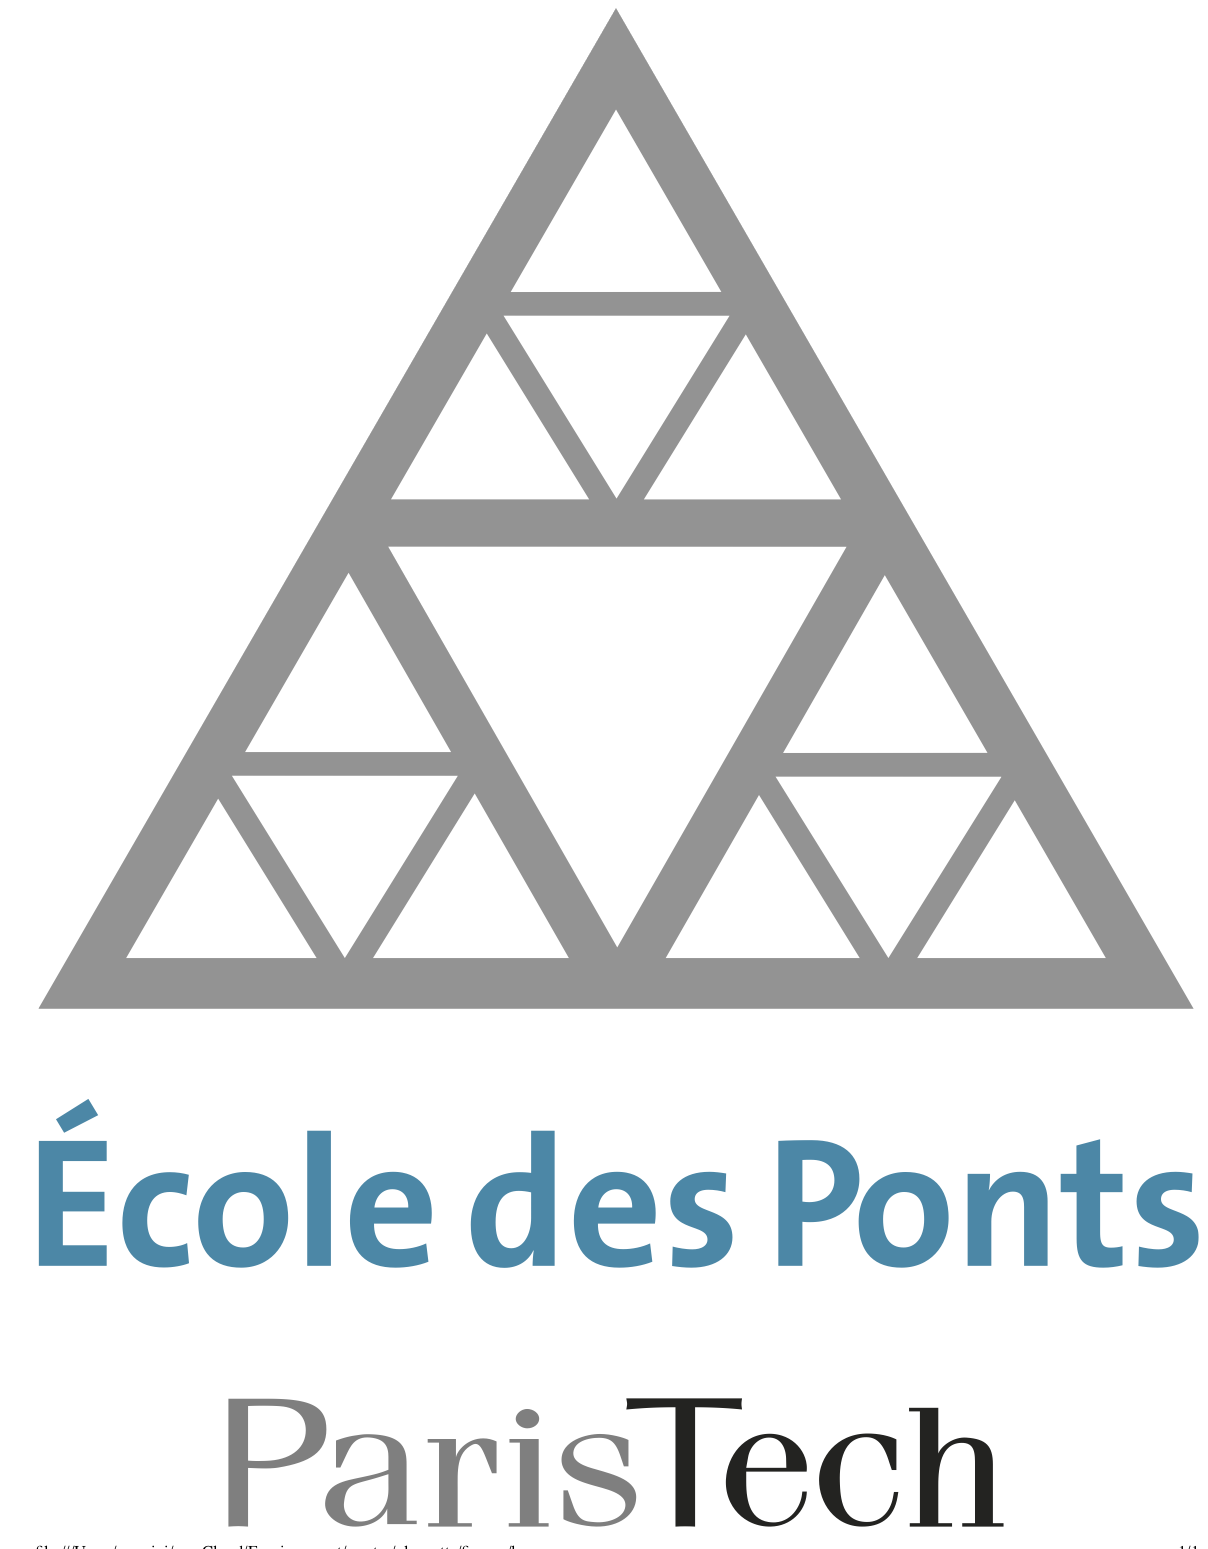
\includegraphics[height=3cm]{figures/logo-enpc.png}
\end{textblock*}%

\vspace*{3cm}
\begin{center}

\large Sorbonne Université et École Nationale des Ponts et Chaussées \medskip
\\


Année Académique  2019-2020\\ 

\end{center}

\vspace*{3cm}
\begin{center}
\LARGE Master de Mécanique\\
Mécanique des Solides:
 Matériaux et  Structures
\end{center}
\noindent\vspace*{3cm}
\begin{center}
\textbf{\Large Présentation et catalogue des cours}\\
\today\\

\end{center}


\vfill

\begin{flushleft}
\begin{tabular}{l}
Responsable Sorbonne Université\\ 
Corrado MAURINI
corrado.maurini@sorbonne-universite.fr\medskip\\
Responsable ENPC\\
Karam SAB karam.sab@enpc.fr
\end{tabular}
{}\end{flushleft} 

\end{titlepage}
\setcounter{tocdepth}{2}
%\dominitoc \dominilof \dominilot
\begin{tableofcontents}
%\dominitoc\dominitoc%\listofmyequations
\end{tableofcontents}
\newpage
\section{Présentation}

\pagestyle{fancy}
\fancyhead[L]{}
\fancyhead[R]{Mécanique des Solides: Matériaux et Structures}
\fancyfoot[C]{\thepage}

Le parcours-type \textbf{Mécanique des Solides: Matériaux et Structures}
du \textbf{Master de Mécanique} est organisé en partenariat entre \href{https://www.sorbonne-universite.fr}{Sorbonne
Université} et 
l'\href{https://www.enpc.fr}{Ecole des Ponts ParisTech}. 
La formation est
étroitement adossée à deux laboratoires de recherche et aux Ecoles Doctorales associées:

\begin{itemize}
\item
  l'\href{http://www.dalembert.upmc.fr}{Institut Jean le Rond d'Alembert} (Unité Mixte de Recherche Sorbonne
  Université -~ CNRS 7190) rattaché à l'Ecole Doctorale Sciences Mécaniques, Acoustique, Electronique et Robotique (\href{http://www.ed391.upmc.fr}{SMAER}) de
  Sorbonne Université.
\item
  Le \href{https://navier.enpc.fr/}{Laboratoire Navier} de l'ENPC 
  rattachée à l'Ecole Doctorale 531 Sciences, Ingénierie et Environnement 
  (\href{http://www.univ-paris-est.fr/fr/-ecole-doctorale-sciences-ingenierie-et-environnement-sie-ed-531-/
}{SIE}) de
  l'Université de Paris-Est.
  

\end{itemize}
L'équipe pédagogique est constituée d'enseignants-chercheurs et chercheurs
des deux laboratoires et d'enseignants-chercheurs de
renommée internationale d'autres laboratoires franciliens de
Mécanique, ainsi que d'industriels spécialistes de la conception et du
calcul de structures mécaniques et de partenaires internationaux. %La
%formation est rattachée aux Écoles Doctorales SMAER de Sorbonne
%Université et à \ldots{}.



\subsection{Objectifs pédagogiques}

Ce parcours a pour objectif de former des spécialistes en mécanique des
solides ayant une très bonne maîtrise des concepts et des outils de
modélisation et simulation des structures mécaniques et des matériaux
constituants. 
Les enseignements délivrent des connaissances sur le
comportement non linéaire des matériaux, la modélisation micro-mécanique,
l'homogénéisation, la dynamique des structures, les méthodes de calcul
numériques (éléments finis) dans le contexte linéaire et  non linéaire, la
modélisation des phénomènes de rupture, endommagement, fatigue ou
d'instabilité dans les solides. 
Ces sujets sont au cœur des préoccupations actuelles des industriels, des problématiques posées par la recherche et développement technologique dans le court et moyen terme et des problématiques de recherche du secteur dans le long terme.


Les enseignements proposés comprennent des unités à caractère fondamental et des unités plus spécialisées, pouvant permettre aussi bien une insertion professionnelle, qu'une poursuite en doctorat. L'objectif de la formation est donc double :
\begin{itemize}
\item Former des spécialistes en calcul des structures, ayant une excellente maîtrise des logiciels industriels et répondant dès leur sortie aux besoins modernes des grandes ou moyennes entreprises chargées de concevoir ou de contrôler des structures industrielles sollicitées mécaniquement.

\item Permettre à l'étudiant, qui le souhaiterait, de s'intégrer aux équipes de recherche les plus performantes dans les domaines du comportement des matériaux et du calcul des structures, que ce soit dans les laboratoires universitaires ou dans l'industrie, en lui donnant une formation conceptuelle moderne et de haut niveau. 
\end{itemize}


Les domaines d'application sont très variés, incluant par exemple les
transports, l’aéronautique, l'aérospatiale, l'énergie, le génie civil, la biomécanique et la robotique.



\paragraph{Mots clés:}
Endommagement, Rupture, Fatigue, Grandes déformations, Élasticité linéaire, Hyperelasticité,
 Viscoélasticité, Poutres, Plaques, Coques, 
Non-linéarités, Stabilité des structures,  Meta-matériaux,  Matériaux,  Matériaux composites,
 Matériaux intelligents,
Éléments finis, Calcul des structures,  Méthodes numériques, Programmation,
Structures, Optimisation, Dynamique des structures
Multi-échelle, Milieux périodiques, 
Formulations Variationnelles, Méthodes approchées, Méthodes asymptotiques,    Méthodes Énergétiques, Génie Civil, Génie Mécanique,
Aéronautique, Aérospatial, Énergies renouvelables,  
Nucléaire, Robotique. 
\subsection{Débouchés professionnels}

Les principaux débouchés professionnels sont :

\begin{itemize}


\item
  Les départements \emph{Calcul}, \emph{Structures} ou \emph{Mécanique}
   des directions R\&D des grands groupes industriels des secteurs aéronautique,
  automobile, génie civil, espace, nucléaire, transports, énergie,...
  (EDF,  CEA, Safran, Framatome, Renault, PSA, EADS, Dassault Aviation, Technip,
  IFP, SNCF, CETIM, Lafarge, ANDRA, Total, ...)

\item Les moyennes entreprises ou start-ups de haute technologie nécessitant des experts en calcul et modélisation des matériaux et des structures pour la conception et l'optimisation des produits, l'élaboration de matériaux innovants, les outils de l’investigation physique des matériaux.

\item L’industrie cimentière, les bureaux d'études spécialisés dans les constructions et les ouvrages du Génie Civil.

\item   Les sociétés de service en informatique spécialisées dans le
  développement de logiciels de simulation numérique 
  et/ou dans la sous traitance auprès des grands groupes.
  
\item
  La poursuite en thèse pour une carrière de recherche académique ou industrielle.
  Les thèses s'effectuent dans le cadre de partenariats entre des
laboratoires universitaires et de grands groupes industriels sous
financement CIFRE ou avec des bourses de thèse proposées par le
Ministère de la Recherche, le CNRS ou des grands Centres de Recherche
(IFSTTAR, CEA, ONERA, IFREMER, \ldots).
\end{itemize}





\section{Information pratiques}
\subsection{Conditions d'admission, pré-requis}

Le Master en Mécanique des Solides vise a créer une communauté intégrée
d'étudiants de haut niveau provenant de parcours variés~:

\begin{itemize}
\item
  Formation universitaire au niveau M1 en Mécanique des Solides 
\item
  Les grandes écoles d'ingénieurs françaises
\item
  Diplômés d'autres universités françaises et internationales
  d'excellent niveau
\end{itemize}
Les pre-réquis pour l’admission sont les suivants:
\begin{itemize}
\item
  Être titulaire d'un Master 1 en Mécanique, Physique, ou Mathématiques
\item
  Être titulaire d'un diplôme d'ingénieur avec des connaissances
  validées en Mécanique, Physique, ou Mathématiques
\end{itemize}
Les candidatures relevant de parcours atypiques, qui ne rentrent pas dans les cas 
mentionnés ci-dessus, seront étudiées avec une attention particulière donnée à l'excellence du niveau en Mécanique, Physique ou Mathématiques.


\subsection{Procédure de candidature}
%
%
\begin{itemize}
  \item
  Les candidatures doivent être déposées sur  le sites de l'une des deux institutions partenaires:
\begin{itemize}
  \item Sorbonne Université: \burl{http://master.spi.sorbonne-universite.fr}
  \item ENPC: \burl{https://www.enpc.fr/masters}
\end{itemize}
Les étudiants doivent exprimer au moment de la candidature des vœux classés pour les trois thématiques possibles (AMMS, DMS, MS).

\item Les étudiants en Master 1 à Sorbonne Université doivent candidater sur le site de Sorbonne Université.

\item Les étudiants en formation d'ingénieur à l'ENPC doivent candidater sur le site de l'ENPC.

\item Les étudiants d'autre provenance peuvent déposer leur candidature sur le sites de l'une des deux institutions partenaires. Nous recommandons de 
déposer la candidature sur le site de Sorbonne Université pour une candidature avec la thématique MS en premier vœux et sur le site de l'ENPC pour une candidature avec la thématique AMMS en  premier vœux.

\item Le diplôme est délivré par l’établissement d’inscription. 

\item La sélection des dossiers est basée sur la qualité du dossier académique 
et du projet pédagogique et professionnel du candidat.  


\end{itemize}

\subsection{Lieux d'enseignement}

En fonction des jours et des options, les enseignements auront lieu sur les campus des deux établissements partenaires:
\begin{itemize}
\item
  Sorbonne Université, \href{https://www.openstreetmap.org/#map=17/48.84691/2.35506}{Campus Pierre et Marie Curie}, 4 place Jussieu, 75005 Paris. Accès: \url{https://www.sorbonne-universite.fr/acces-aux-campus}.
\item
  Ecole des Ponts ParisTech, \href{https://www.openstreetmap.org/search?query=%208%20avenue%20Blaise-%20Pascal%20%20-%20Cité%20Descartes%20-%20Champs-sur-Marne%20#map=18/48.84171/2.58699}{Campus de Marne-la-Vallée}, 
6 et 8 avenue Blaise Pascal, Cité Descartes,
Champs-sur-Marne, 77455 Marne-la-Vallée. Accès: \url{http://www.enpc.fr/venir-lecole}
\end{itemize}

\newpage


\section{Organisation et structuration de la formation}

\subsection{Thématiques}
La parcours-type \emph{Mécanique des Solides: Matériaux et Structures} du
\emph{Master en Mécanique} est structuré en trois \textbf{thématiques}:

\begin{itemize}
\item
  \textbf{AMMS: Analyse Multi-échelle des Matériaux et des Structures\\
  }Responsables : Eric Lemarchand et Karam Sab (ENPC)\\
  Capacité: 15 étudiants environ. 
\item
  \textbf{DMS: Durabilité des Matériaux et des Structures}\\
  Responsable: Alain Ehrlacher (ENPC)\\
  Capacité: 15 étudiants environ. 
\item
  \textbf{MS: Modélisation et Simulation}\\
  Responsables Corrado Maurini et Hélène Dumontet (Sorbonne Université)\\
  Capacité: 35 étudiants environ. 
\end{itemize}


\subsection{Organisation des enseignements}

\noindent La formation, de 60 ECTS\footnote{\emph{European Credit Transfer and Accumulation System},  voir
\burl{https://en.wikipedia.org/wiki/European_Credit_Transfer_and_Accumulation_System} ou \burl{https://ec.europa.eu/education/resources-and-tools/european-credit-transfer-and-accumulation-system-ects_en}
}, s'articule sur deux semestres:
\begin{itemize}
\item Le \textbf{premier semestre (30 ECTS)} de mi-septembre à fin février inclut:

\begin{itemize}
\item
\textbf{12 ECTS} de \textbf{Tronc Commun (TC)} avec  4 cours de 3 ECTS parmi 6 cours offerts.
\item
  \textbf{12 ECTS} d'enseignements de la \emph{thématique}.
\item
  \textbf{6 ECTS} d'enseignements \emph{électifs}.
\end{itemize}
\item Le \textbf{second semestre (30 ECTS)} est constitué par un stage de 6 mois dans
une entreprise ou un laboratoire de recherche, valorisé pour 27 ou 30
ECTS. Un cours de langue (3 ECTS) peut compléter la formation en fonction du parcours de l'étudiant.
\end{itemize}

Les étudiants peuvent, s'ils le souhaitent, suivre des cours optionnels supplémentaires, qui seront comptabilisés en plus des 60 ECTS obligatoires et reportés dans le supplément au diplôme.

\subsection{Tronc Commun}
Les enseignements du tronc commun sont dispensés de mi-septembre à décembre. 
Ils s'adressent aux étudiants des trois thématiques et ont pour ambition 
d'être les cours de référence pour la formation de l'étudiant en mécanique des matériaux et des structures. 
La compatibilité de l'emploi du temps est assurée entre les six cours de tronc commun.
 \begin{enumerate}
  \item  Introduction à l’homogénéisation en mécanique des milieux continus  (3 ECTS, responsable K.~Sab)
  \item  Mécanique de la rupture fragile (3 ECTS, responsable J.B.~Leblond)
  \item  Comportements non-linéaires des solides (3 ECTS, responsable D.~Kondo)
  \item  Endommagement (3 ECTS, responsables J.~Bleyer/H.~Dumontet)
  \item Calcul numérique des solides et structures non linéaires
    (3 ECTS, responsables D.~Duhamel/C.~Maurini)
  \item  Fatigue (3 ECTS, responsable M.~Peigney)

  \end{enumerate}
Chaque thématique recommande aux étudiants de suivre quatre cours  parmi les six ci-dessus. 

\subsection{Dates clés}
\begin{itemize}
\item Remise à niveau: deuxième semaine de septembre.
\item Première période de cours: troisième semaine de septembre - décembre.
\item Deuxième période de cours: décembre - février.
\item Stage: mars - septembre, avec soutenances en septembre.
\end{itemize}

\subsection{Stage}
Le stage de fin d'étude, d'une durée de 4 à 6 mois, doit permettre à l'étudiant de mettre en application l’ensemble des connaissances acquises durant sa formation et acquérir des compétences additionnelles spécialisées dans un domaine d'application précis ou en 
matière d’initiation à la recherche. 

\begin{itemize}
\item Le stage  se déroulera  dans une entreprise ou dans le contexte d'un laboratoire de recherche en France ou à l'étranger. Les stages en entreprise ont généralement lieu dans des bureaux calculs ou R\&D des grands groupes industriels ou organismes partenaires de la formation, mais ils peuvent aussi se dérouler dans des petites ou moyennes entreprises de haute technologie ou dans des bureaux d'études spécialisés dans les constructions ou les ouvrages du Génie Civil (voir \emph{Débouchés professionnels}). 
\item Le stage est valorisé à la hauteur de 27 ou 30 ECTS, en fonction du parcours de l'étudiant. L'évaluation du stage se fait sur la base d'un rapport écrit, de l'avis de l'encadrant et d'une soutenance orale ayant lieu à la fin de l'année académique (mi-septembre).
\end{itemize}
Pour les stages industriels ou académiques, les étudiants pourront bénéficier des nombreux contacts des deux laboratoires de recherche, en France (EDF, Safran, Framatome, Dassault, Renault, PSA, EADS, CETIM, Lafarge, Andra, Total) et à l'international, incluant les meilleures universités à l'échelle mondiale (\emph{e.g.} Caltech, Cambridge, Oxford, ETH, EPFL, KTH, La Sapienza, Politecnico di Milano, Louisiana State University, etc.)
%Des exemples  incluant au niveau academique Caltech, Lousiana State University,Université La Sapienza, )
\newpage
%-------------------------------------------------
\section{Thématique Analyse Multi-échelle des Matériaux et des Structures (AMMS)}
%-------------------------------------------------
 A travers les différents cours proposés dans cette thématique, on souhaite former les étudiants à la modélisation mécanique des matériaux et des structures en intégrant  les propriétés de leurs différents constituants et les informations sur leur agencement à différentes échelles de l'espace. Les applications des différentes démarches d'analyse présentées dans l'ensemble des cours concernent les domaines du Génie Civil, du Génie Mécanique et plus largement de l'Industrie. On s'intéressera plus particulièrement aux matériaux cimentaires, aux géomatériaux (sols, roches) et aux structures multi-couches (fibre-résine, bois lamellé-collé, acier-élastomère). Cette  formation par la recherche répond pleinement aux exigences d'une candidature à la réalisation d'un travail de doctorat en Mécanique et Structures, mais elle constitue également un complément de formation sur des thématiques de recherche d'actualité susceptible d'intéresser de futurs ingénieurs.

\subsection{Unités d'enseignements de la thématique}
\begin{itemize}
\item
  \textbf{12 ECTS Tronc Commun.} Les cours de TC obligatoires pour cette thématique sont:

  \begin{itemize}
  \item
    Mécanique de la rupture (3 ECTS, TC)
  \item
    Comportements non-linéaires des solides (3 ECTS, TC)
  \item
    Calcul numérique des solides et structures non-linéaires (3 ECTS, TC)
  \item
    Introduction à l’homogénéisation en mécanique des milieux continus (3 ECTS, TC)
  \end{itemize}
\item
  \textbf{12 ECTS de spécialisation}

  \begin{itemize}
  \item
   Elasticité et résistance des matériaux hétérogènes (3 ECTS, AMMS)
  \item
    Micro-poro-mécanique appliquée (3 ECTS, AMMS)
  \item
    Modélisation des structures multi-couches (3 ECTS, AMMS)
  \item
    Images et mécanique (3 ECTS, AMMS)
  \end{itemize}
\item
  \textbf{6 ECTS électifs}

  \begin{itemize}
  \item
    Endommagement (3 ECTS, TC)
  \item
    Approches multi-échelles de la plasticité des métaux/Durabilité des
    bétons (3 ECTS, DMS)
  \item
    Homogénéisation en calcul à la rupture (3 ECTS, AMMS)
  \item
    Méthodes d'identification des paramètres de modèles (3 ETCS, AMMS)
  \end{itemize}
\
\end{itemize}

\noindent Légende: (TC) Cours du Tronc Commun; (AMMS) Cours propres à la thématique AMMS; (DMS) Cours propres à la thématique DMS. Voir le Catalogue des cours pour les détails.
\newpage
\subsection{Contacts}

\subsubsection{Responsables de la thématique MS}
\begin{itemize}

\item Karam Sab\\
Directeur de Recherche\\
Laboratoire Navier - ENPC\\
6 et 8 Avenue Blaise Pascal\\
Cité Descartes\\
77455 CHAMPS SUR MARNE\\
Tél : 01.64.15.37.49\\
Mail : \href{mailto:karam.sab@enpc.fr}{karam.sab@enpc.fr}\\

\item Eric Lemarchand\\
Chargé de Recherche\\
Laboratoire Navier - ENPC\\
6 et 8 Avenue Blaise Pascal\\
Cité Descartes\\
77455 CHAMPS SUR MARNE\\
Tél : 01.64.15.36.58\\
Mail : \href{mailto:eric.lemarchand@enpc.fr}{eric.lemarchand@enpc.fr}\\


\item 
Alice Tran \\
Adjointe administrative \\
ENPC \\
6 et 8 Avenue Blaise Pascal \\
Cité Descartes\\
77455 CHAMPS SUR MARNE\\
Tél : 01.64.15.36.84 \\
Mail : \href{mailto:alice.tran@enpc.fr}{alice.tran@enpc.fr} \\
\end{itemize}


\newpage
\section{Thématique Durabilité des Matériaux et des Structures (DMS)}
La thématique Durabilité des Matériaux et des Structures  vise a former des personnels de haut niveau scientifique, susceptibles de prendre en charge les problématiques de durabilité des installations futures et d'identification de l'état des installations existantes afin de déterminer la durée de vie résiduelle et de décider d'éventuels renforcements ou d'optimiser une politique de maintenance.
Les aspects prise en compte de l'aléas et analyse des conséquences éventuelles d'un accident seront particulièrement étudiés.
Les applications concerneront les ouvrages d'art (Ponts, tunnels,  routes, \ldots), les ouvrages pour la production ou le stockage d'énergie (Barrages, STEP, réacteurs nucléaires à eau pressurisée, éoliennes offshore ou on shore, \ldots) et les bâtiments.
A l'issue de la formation les étudiants maîtriseront les principaux modèles de vieillissement des matériaux et des structures, sauront mettre en oeuvre une démarche d'identification de l'état d'une structure ancienne, connaîtront les principales méthodes pour la prise en compte de l'aléas des matériaux, des chargements ou lié à l'ignorance de la connaissance précise de l'état d'une structure.
Ils sauront en déduire une probabilité d'accident ou de durée de vie d'un ouvrage et poser rationnellement un problème d'optimisation d'une politique de renforcement ou de maintenance.
Les débouchés de cette formation pourrait être une thèse dans un laboratoire de recherche ou un poste dans un centre de recherche ou un bureau d'études industriel ou de génie civil prenant en charge l'étude de la durée de vie résiduelle des structures, des renforcements d'ouvrages ou d'optimisation des politiques de maintenance. 

\subsection{Unités d'enseignements de la thématique}
\begin{itemize}
\item
  \textbf{12 ECTS Tronc Commun.} Les cours de TC obligatoires pour cette thématique sont:

  \begin{itemize}
  \item
    Mécanique de la rupture (3 ETCS, TC)
  \item
    Endommagement (3 ETCS, TC)
  \item
    Fatigue (3 ETCS, TC)
  \item
    Introduction à l’homogénéisation en mécanique des milieux continus (3 ETC, TC)
  \end{itemize}
\item
  \textbf{12 ECTS de spécialisation}

  \begin{itemize}
  \item
    Enjeux des accidents nucléaires graves / Séminaire «~Enjeux de
    l'électricité dans les systèmes énergétiques~» (3 ECTS, DMS)
  \item
    Physique et exploitation des REP (3 ECTS, DMSE)
  \item
    Identification et suivi en service des structures de génie civil et
    des grands systèmes (3 ECTS, DMS)
  \item
    Ingénierie des incertitudes en mécanique (3 ECTS, DMS)
  \end{itemize}
\item
  \textbf{6 ECTS électifs}

  \begin{itemize}
  \item
    Approches multiéchelles de la plasticité des métaux/Durabilité des
    bétons (3 ECTS, DMS)
  \item
    Modélisation et simulation des équipements des structures:
    application à l'analyse sismique (3 ECTS, DMS)
  \item
    Autres cours des parcours AMMS, MS et du TC.
  \end{itemize}
\end{itemize}
\noindent Légende: (TC) Cours du Tronc Commun; (MS) Cours propres à la thématique MS; (AMMS) Cours propres à la thématique AMMS; (DMS) Cours propres à la thématique DMS. 
\subsection{Contacts}
\subsubsection{Responsables de la thématique DMS}
\begin{itemize}
\item  
Alain Ehrlacher\\ 
Président du département Génie Mécanique et Matériaux \\ENPC 6 et 8 Avenue Blaise Pascal\\
Cité Descartes \\
77455 CHAMPS SUR MARNE \\
Tél : 01.64.15.37.17 \\
Mail : \href{mailto:alain.ehrlacher@enpc.fr}{alain.ehrlacher@enpc.fr}

\item
Alice Tran Adjointe administrative ENPC\\
6 et 8 Avenue Blaise Pascal Cité Descartes \\
77455 CHAMPS SUR MARNE \\
Tél : 01.64.15.36.84 \\
Mail : \href{mailto:alice.tran@enpc.fr}{alice.tran@enpc.fr}
\end{itemize}
\newpage


%-------------------------------------------------
\section{Thématique Modélisation et Simulation (MS)}
%-------------------------------------------------
%\subsection{Présentation}


La Thématique \emph{Modélisation et Simulation} a pour vocation de délivrer une formation approfondie en modélisation et simulation numérique des phénomènes physiques rencontrés dans le domaine de la mécanique des solides.
L'étudiant diplômé possèdera une solide maîtrise des concepts de mécanique des milieux continus, une bonne connaissance des grandes classes de matériaux, une formation aux méthodes avancées en mécanique de la rupture et de l'endommagement, des bonnes connaissances sur les méthodes de résolution numérique de problèmes linéaires et non linéaires, ainsi qu'une pratique opérationnelle de la simulation sur ordinateurs.

Parmi les cours de spécialisation, le module \emph{Pratiques de codes de calculs des structures et applications} (obligatoire) a pour but de développer la pratique numérique des concepts et méthodes introduits dans les cours de tronc commun et de former les étudiants à l'utilisation avancée des codes de calculs de structures utilisés en contexte industriel ({Abaqus}) sur les problèmes de plasticité, homogénéisation, rupture, couplages multiphysiques, calculs non-linéaires. Ce module aura lieu en parallèle des cours de tronc commun.
Les autres options de spécialisation  sont au choix parmi des sujets spécifiques à la thématique (\emph{composites} ou \emph{stabilité des structures}),  un \emph{projet} encadré en groupes  sur un sujet industriel ou académique, ou une ouverture vers le \emph{couplage fluides-structures en biomécanique}, mutualisé avec le Master en Mécanique des Fluides et Computational Mechanics de Sorbonne.

\subsection{Unités d'enseignements de la thématique}
\begin{itemize}
\item
  \textbf{12 ECTS de Tronc Commun.} 

  \begin{itemize}
  \item
    Mécanique de la rupture (3 ECTS, TC)
  \item
    Comportements non-linéaires des solides (3 ECTS, TC)
  \item
    Calcul numérique des solides et structures non-linéaires (3
    ECTS, TC)
  \item
    Introduction à l’homogénéisation en mécanique des milieux continus (3 ECTS, TC)
  \end{itemize}
\item
  \textbf{12 ECTS de spécialisation dont}

  \begin{itemize}
  \item
    Pratiques de codes de calculs des structures et applications (6 ECTS, MS)
  \item
    6 ECTS avec deux unités de 3 ECTS au choix parmi

    \begin{itemize}
    \item
      Structures composites: conception et optimisation (3 ECTS, MS)
    \item
      Stabilité des structures (3 ECTS, MS)
    \item
      Projet en calcul non-linéaire des structures (3 ECTS, MS)
    \item
      Interaction fluides-structures avec applications à la biomécanique et au bio-inspiration (3 ECTS, MS)
    \end{itemize}
  \end{itemize}
\item
  \textbf{6 ECTS électifs}

  \begin{itemize}
  \item
    Elasticité et résistance des matériaux hétérogènes (AMMS - 3 ECTS)
  \item
    Approches multi-échelles de la plasticité des métaux (DMS - 3 ECTS)
  \item
    Endommagement (TC - 3 ECTS)
  \item
    Fatigue des matériaux et des structures (TC - 3 ECTS)
  \end{itemize}
\end{itemize}

\noindent Légende: (TC) Cours du Tronc Commun; (MS) Cours propres à la thématique MS; (AMMS) Cours propres à la thématique AMMS; (DMS) Cours propres à la thématique DMS. 
\newpage
\subsection{Contacts}
\subsubsection{Secrétariat pédagogique de la thématique MS}

Vanessa Teixeira\\
E-mail : \href{vanessa.teixeira@sorbonne-universite.fr}{vanessa.teixeira@sorbonne-universite.fr}


\subsubsection{Responsables de la thématique MS}
\begin{itemize}
  \item 
Corrado Maurini\\
Professeur des Universités \\
Sorbonne Université\\
Institut Jean Le Rond d'Alembert (UMR 7190)\\
Tour 55-65, bureau 412 (4ème étage)\\
4 Place Jussieu, case 162 | 75242 Cedex 05 Paris\\
Tél: 01 44 27 87 19\\
Web: \url{http://www.lmm.jussieu.fr/~corrado}\\
E-mail: \href{mailto:corrado.maurini@sorbonne-universite.fr}{corrado.maurini@sorbonne-universite.fr}\\

\item Hélène Dumontet\\
Professeur des Universités \\
Sorbonne Université\\
Institut Jean Le Rond d'Alembert (UMR 7190)\\
Tour 55-65, bureau 312 (3ème étage)\\
4 Place Jussieu, case 162 | 75242 Cedex 05 Paris\\
Tél: 01.44.27.87.00 \\
E-mail : \href{mailto:helene.dumontet@sorbonne-universite.fr}{helene.dumontet@sorbonne-universite.fr}
 
\end{itemize}

\newpage
\section{Catalogue des cours du Tronc Commun}
\setlength{\itemsep}{0pt}\small
\newcommand{\courstitle}[1]{\subsection{#1}}
\subsection{Introduction à l’homogénéisation en mécanique des milieux continus }

\paragraph{Professeur:\newline} 
Karam Sab, \url{https://navier.enpc.fr/SAB-Karam}, E-Mail : 
karam.sab@enpc.fr



\paragraph{Objectifs de l'Unité d'Enseignement: }
Le comportement des matériaux peut être modélisé de deux manières complémentaires : la démarche phénoménologique et le changement d'échelle. L'approche phénoménologique consiste à identifier expérimentalement des lois de comportement à l'échelle d'un élément de volume représentatif du matériau, alors que les techniques de changement d'échelle se proposent de calculer des estimations du comportement du matériau à partir du comportement de ses constituants et de leurs fractions volumiques. L'objet de ce cours est d'introduire les concepts et techniques de base nécessaires pour effectuer, grâce au changement d’échelle, une homogénéisation d’un matériau hétérogène élastique linéaire.

\paragraph{Contenu de l’Unité d’Enseignement:}

\begin{itemize}
	\item Introduction des différentes échelles d'observation dans les solides hétérogènes. Notion de Volume Élémentaire Représentatif (VER).
	\item Conditions aux limites homogènes en déformation ou en contrainte. Tenseurs d'élasticité et de souplesse du VER.
	\item Bornes de Voigt et de Reuss. Cas du composite unidirectionnel.
	\item Méthodes approchées dans le cas de faibles concentrations d'inclusions. Aperçu des méthodes autocohérentes et du modèle de Mori-Tanaka.
	\item Cas des milieux à structure périodique.
\end{itemize}

\paragraph{Mots-clés:} 

Homogénéisation. Milieux périodiques. Micromécanique.



\paragraph{Pré-requis: }

Il est nécessaire de maîtriser la modélisation élastique linéaire des solides déformables

\paragraph{Compétences développées dans l’unité:}
Pratique de la modélisation en élasticité linéaire. Homogénéisation des matériaux élastiques.


\paragraph{Références bibliographiques:}
\begin{enumerate}
\item Hashin Z., Analysis of composite materials, a survey. J. Appl. Mech., 50, 481-505 (1983); 
\item Sanchez-Hubert J., Sanchez-Palencia E., Introduction aux méthodes asymptotiques et à l’homogénéisation, Masson, Paris, 1992; 
\item Sab K., On the homogenization and simulation of random materials. Eur. J. Mech. A/Solids, 11 (5), 585-607. 1992; 
\item Nemat-Nasser S., Hori M., Micromechanics: Overall Properties of Heterogeneous Materials, North-Holland, 1993; 
\item Kozlov S.M., Olenik O., Zhikov V., Homogenization of Differential Operators, Springer Verlag,1994; 
\item Sab K., Propriétés homogénéisées des matériaux hétérogènes élastiques: définition et bornes. Actes des journées “ changement d’échelle ”. 7 et 8 juin 2000. Nantes. LCPC. 2000;
\item 
Bornert M., Bretheau T., Gilormini P. (Eds), Homogénéisation en mécanique des matériaux, Hermes, Paris, 2001.
\end{enumerate}\newpage
\subsection{Mécanique de la rupture fragile}

\paragraph{Professeur:} 
Jean-Baptiste Leblond, \url{http://www.dalembert.upmc.fr/home/leblond},\\ E-Mail: jbl[arobas]lmm[dot]jussieu[dot]fr


\paragraph{Objectifs de l'Unité d'Enseignement:}
Exposer les bases de la théorie de la rupture fragile, telle qu’elle est couramment utilisée dans les laboratoires de recherche et l’industrie de pointe (nucléaire, aéronautique, …) pour prédire et maîtriser la fissuration des matériaux.


%\emph{English : Expound the bases of the theory of brittle fracture mechanics, such as currently used in research institutions and high-tech industries (aeronautical, nuclear…) in order to predict and master cracking of materials.}


\paragraph{Contenu de l’Unité d’Enseignement:}
Le cours inclut 2 chapitres sur les connaissances de base et un 3ème un peu plus spécialisé: : 
\begin{itemize}
 \item Théorie d’Irwin du KIc,
 \item Théorie énergétique de Griffith,
 \item Propagation de fissures en mode mixte.
\end{itemize}

\paragraph{Pré-requis:}

\begin{itemize}
\item Mécanique des solides niveau Master 1 (niveau d'exigence 100\%)
\item Bonnes bases de mathématiques pratiques (algèbre et analyse élémentaires, équations différentielles, fonctions d’une variable complexe, calculs). (niveau d'exigence 50\%).
\end{itemize}

\paragraph{Mots clés:}
Matériaux élastiques, fissuration, singularités de contraintes, critère de propagation, approche énergétique, mode mixte, branchement de fissures

\paragraph{Compétences développées dans l’unité:}
A l’issue de l’UE, l’étudiant(e) dispose des outils de base de la mécanique de la rupture fragile, exposés de manière exhaustive et détaillée, lui permettant soit de satisfaire aux exigences d’un bureau d’études en mécanique soit d’entreprendre une thèse dans le domaine. \newpage
\subsection{Comportements non-linéaires des solides}

\paragraph{Professeur(s):} Djimedo Kondo, \url{http://www.dalembert.upmc.fr/home/kondo/}.\newline E-Mail: djimedo.kondo@sorbonne-universite.fr.
%Cet enseignement vise à donner aux étudiants un cadre unifié pour la formulation des lois de comportements mécaniques non linéaires, et à leur considération dans le con-texte du calcul de structures. Le point de vue adopté est pour l’essentiel macrosco-pique et phénoménologique, avec cependant des éléments de micromécanique des matériaux qui viennent justifier ou enrichir ce point de vue. 
%Après un rappel des différentes classes de lois de comportements thermomécaniques non linéaires, on présentera le cadre thermodynamique des processus irréversibles, l’objectif principal étant la formulation de lois de comportements régis par des méca-nismes dissipatifs identifiés. Le rôle clef des 2 principes de la thermodynamique, et notamment de l’inégalité de Claussius-Duhem qui en résulte, sera souligné. 
%Suivra un exposé du cadre des Matériaux Standards généralisés (MSG) pour lequel la formulation des lois constitutives repose sur :
%\begin{itemize}
%\item un choix éclairé des variables d’état incluant les variables internes correspondant aux types de comportements considérés
%\item  l’introduction d’un potentiel thermodynamique (en général l’énergie libre d’Helmholtz), fonction de l’ensemble des variables d’état et décrivant l’état thermo-dynamique du matériau
%\item  le choix d’un potentiel de dissipation fournissant les lois d’évolution des variables internes. 
%\end{itemize}

%Ce cadre des MSG servira ensuite à construire et étudier de manière unifiée les grandes classes de modèles de comportements thermomécaniques, allant de la ther-moélasticité à la thermo-elastoviscoplasticité. On évoquera brièvement la mécanique de l’endommagement. 
%Seront également décrites les équations régissant les évolutions thermo-mécaniques, nécessitées par la résolution de problèmes de structures qui jalonneront l’ensemble de l’enseignement. Ceci sera systématiquement complété par l’exposé du cadre variationnel associé.

\paragraph{Contenu de l’Unité d’Enseignement:}
\begin{itemize}
\item	Bref rappel des concepts de base de la mécanique des milieux continus, et des divers comportements des matériaux de structure
\item	Lois de bilan en thermomécanique des milieux continus : bilan de quantité de mouvement, bilan d’énergie et bilan d’entropie. Présentation de l’inégalité de Clausius-Duhem, et des dissipations (intrinsèque et thermique)
\item	Cadre des matériaux standards généralisés : méthode générale de formulation des lois de comportement; rôle de l’Inégalité de Clausius-Duhem. Notions de variables d’état, de variables internes, de fonctions d’état et de potentiels thermodynamiques. Equation de la chaleur.
Construction et identification des grandes classes de modèle de comportement : rappels des modèles rhéologiques fondamentaux à base de ressort, patin et amortis-seur. Cas des matériaux thermoplastiques, des matériaux thermo-viscoélastiques (mo-dèle de Kelvin-Voigt, modèle de Maxwell)
\item	Elastoplasticité et applications : Formulation de modèles élastoplastiques par-faits. Prise en compte de l’écrouissage (isotrope et/ou cinématique). Calculs thermo-mécaniques et résolution de problèmes simples de structures élastoplastiques.
\item	Quelques notions sur des lois couplant élasticité et endommagement isotrope
\item	Comportements Elastoviscoplastiques : Présentation de quelques modèles de com-portement dépendant du temps; effet régularisant de la viscosité. 
\end{itemize}



\paragraph{Références bibliographiques}:

\begin{enumerate}
\item 
H. Ziegler, An introduction to thermoechanics, North Holland, 1983
\item P. Germain, Q. S. Nguyen, P. Squat, Continuum Thermodynamics, J. Appl. Mech., ASME 50, 1010-1021, 1983.
\item J. Lemaître, J. L. Chaboche, Mechanics of Solids Materials, Cambridge University Press, 1990
\item G. Maugin, The thermomechanics of plasticity and fracture, Cambridge University Press 1992
\item Q. S. Nguyen, Stability and Nonlinear Solids Mechanics, Wiley, 2000 
\item M. Fremond, Non Smooth Thermomechanics, Springer Verlag, 2002,
\item J. Lubliner, Plasticity Theory. Dover Publications Inc., Mineola, New York, 2008.
\item H. Maitournam, Matériaux et Structures inélastiques, Editions de l’Ecole Polytechnique, 2016 
\end{enumerate}\newpage

\subsection{Calcul numérique des solides et structures non linéaires}

\paragraph{Professeur(s):} 
\begin{itemize}
\item Denis Duhamel, \url{https://www.enpc.fr/denis-duhamel}
\item Corrado Maurini, \url: \url{http://www.lmm.jussieu.fr/~corrado} %\href{mailto:corrado.maurini@sorbonne-universite.fr}{corrado.maurini@sorbonne-universite.fr}
\end{itemize}

\paragraph{Objectifs de l'Unité d'Enseignement: }
L’enseignement a pour but de résoudre des problèmes de mécanique des solides non linéaires sur ordinateur en implémentant la méthode des éléments finis et les algorithmes de résolution. 
Les étudiants seront initiés à l’utilisation des outils modernes de calcul scientifique à haute performance (FEniCS, PETSc) des outils de visualisation (paraview) et de gestion de projet (git).

\paragraph{Contenu de l’Unité d’Enseignement:}

\begin{itemize}
\item Elasticité linéaire, formulation variationnelle, discrétisation:  Rappel sur la résolution d’un problème de mécanique par éléments finis. Prise en main de python et FEniCS, Résolution d’un problème d’élasticité par FEniCS
\item	Elasticité non linéaire:  Elasticité non-linéaire, linéarisation, flambement, stabilité. Résolution d’un problème d’élasticité non linéaire, flambement et post-flambement
\item	Dynamique non linéaire: Méthodes implicite et explicite. Résolution d’un problème de dynamique non linéaire
\item	Projet: travail sur un projet en binôme
\end{itemize}

\paragraph{Pré-requis:}
\begin{itemize}
\item Mécanique des milieux continus
\item Connaissance d’un langage de programmation (idéalment python),
\item Cours de base d’élements finis et méthodes numériques
\end{itemize}


\paragraph{Compétences développées dans l’unité}
\begin{itemize}
\item Capacité de développer un code numérique basé sur la méthode des éléments finis pour résoudre un problème d’élasticité linéaire et non-linéaire en statique ou dynamique en utilisant le language python et la librarie FEniCS
\item Elasticité nonlinéaire,  méthodes explicites et implicites pour la dynamique des structures, étude numérique de bifurcation et stabilité dans le cadre quasi-statique.
\item Introduction aux systèmes de gestion de révision (git), Introduction aux outils de visualisation et maillage, Utilisation des solveurs de systèmes d’équations linéaires et non-linéaires à grande dimension
\end{itemize}

\paragraph{Références bibliographique:}
{\footnotesize
\begin{enumerate}
	\item Belytschko T., Liu W. K. and Moran B., Non linear finite elements for continua and structures, 2000, Wiley. 
 \item Dhatt G., Touzot G. et Lefrancois E., Une présentation de la méthode des éléments finis, 2005, Hermes.
 \item  Holzapfel G.A., Nonlinear solid mechanics, 2000, Wiley.
 \item Scott R., Introduction to Automated Modeling with Fenics, 2018, Computational Modeling Initiative LLC.
 \item Langtange, P. and Logg A., Solving PDEs in Python, 2017, Springer.
 \item Davide Bigoni 
  Nonlinear Solid Mechanics
  Bifurcation Theory and Material Instability, 2012, 
   Cambridge University Press.
 \item Wriggers, P., Nonlinear finite element method, 2008, Springer.
 \item Bonnet M., Frangi A., Rey C., The finite element method in solid mechanics, 2014, McGraw Hill.
\end{enumerate}
}
\newpage
\subsection{Fatigue}

\paragraph{Professeur:} 
Michael PEIGNEY, \url{https://navier.enpc.fr/PEIGNEY-Michael},\newline E-mail: michael.peigney@enpc.fr


\paragraph{Objectifs de l'Unité d'Enseignement:}
La maîtrise par l’ingénieur des problèmes de conception de structures mécaniques exige de connaître et comprendre tous les modes possibles de défaillance. Ce cours cible les modes de défaillance par fatigue, susceptibles d’intervenir pour les structures soumises à des sollicitations variables en temps.
A l’issue de l’Unité d’Enseignant, les étudiants :
(i) connaîtront les concepts de base de la fatigue et de l’accumulation de l’endommagement dans les matériaux et les structures sous chargement cycliques et éventuellement aléatoires;
(ii)	connaîtront les principaux critères utilisés dans le milieu industriel; (iii)	seront capables d’en déduire la durée de vie d’une structure sous  chargement cyclique  
(iv)	sauront expliquer les causes des défaillances constatées en service.




\paragraph{Contenu de l’Unité d’Enseignement:}
\begin{itemize}
\item	\emph{Phénomènes physiques.}
Introduction de la problématique à partir d’un cas pratique: essieu-roue-rail. Mise en évidence du phénomène de fatigue. Courbes de Wöhler. Distinction entre fatigue à faible et à grand nombre de cycles. Mécanismes physiques de la fatigue (plasticité, fissuration, distinction entre amorçage et propagation).

\item	\emph{Chargements cycliques et théorèmes d’adaptation.}
Classification des comportements cycliques en élastoplasticité (adaptation, accommodation, rochet). Théorèmes de convergence aux temps longs. Théorèmes d’adaptation (statique et cinématique). Extensions hors de la plasticité parfaite. 

\item	\emph{Critère de fatigue.} Endurance illimitée
Critère de fatigue à grand nombre de cycles, en chargement uniaxial (parabole de Gerber, droite de Goodman) et multiaxial (notamment critères de Sine, Crossland, Dang Van). 

\item	\emph{Critère de fatigue.} Endurance limitée. Chargements aléatoires 
Lois d’endurance limitée. Durée de vie en fatigue à faible nombre de cycles (loi de Manson-Coffin, critère énergétique). Règles de cumul de Miner. Méthode Contrainte-Résistance. Comptage de type rainflow.


\end{itemize}

\paragraph{Pré-requis:} Mécanique de milieux continus. Des notions de plasticité sont souhaitables.


\paragraph{Compétences développées dans l’unité:}

Compréhension du comportement de structures élasto-plastiques sous chargement cycliques et des modes de défaillance associés, Dimensionnement de structures à la fatigue. 




\paragraph{Références bibliographiques:}
{\footnotesize
\begin{enumerate}

\item Constantinescu, A., K. Dang Van, and M. H. Maitournam. "A unified approach for high and low cycle fatigue based on shakedown concepts." Fatigue \& fracture of engineering materials \& structures 26.6 (2003): 561-568.

\item Bertolino, G., et al. "A multiscale approach of fatigue and shakedown for notched structures." Theoretical and Applied Fracture Mechanics 48.2 (2007): 140-151.

\item Peigney, Michael. "Shakedown theorems and asymptotic behaviour of solids in non-smooth mechanics." European Journal of Mechanics-A/Solids 29.5 (2010): 784-793.

\item Peigney, Michael. "Shakedown of elastic-perfectly plastic materials with temperature-dependent elastic 
moduli." Journal of the Mechanics and Physics of Solids 71 (2014): 112-131. 

\item Papadopoulos, Ioannis V., et al. "A comparative study of multiaxial high-cycle fatigue criteria for metals." International Journal of Fatigue 19.3 (1997): 219-235.

\item Papadopoulos, Ioannis V. (editor) Multiaxial fatigue limit criterion of metals. Springer Vienna, 1999.

\end{enumerate}
}
\newpage
\subsection{Endommagement}

\paragraph{Professeurs:}

\begin{itemize}
\item 
Hélène Dumontet, \url{http://www.dalembert.upmc.fr/home/dumontet},\\ E-mail : \href{mailto:helene.dumontet@sorbonne-universite.fr}{helene.dumontet@sorbonne-universite.fr}

\item
Jérémy Bleyer, \url{https://navier.enpc.fr/BLEYER-Jeremy},\\ E-mail : \href{mailto:jeremy.bleyer@enpc.fr}{jeremy.bleyer@enpc.fr}
\end{itemize}

\paragraph{Objectifs de l'Unité d'Enseignement}
Les objectifs de cet enseignement sont: 
\begin{itemize}
	\item de fournir les bases théoriques de la mécanique de l’endommagement des matériaux quasi-fragiles, en particulier concernant la formulation de lois de comportements macroscopiques couplant  élasticité et endommagement. 
 	\item d’étudier la problématique de l’initiation et de l’évolution de l’endommagement dans un cadre numérique afin d’aborder le caractère mal-posé des modèles d’endommagement locaux puis de proposer une ouverture vers plusieurs techniques de régularisation et les liens vers les modèles de rupture fragile.
\end{itemize}

\paragraph{Contenu de l’Unité d’Enseignement}
Après une brève introduction sur l’origine microscopique de l’endommagement comme processus faisant évoluer les propriétés macroscopiques des matériaux, les séances de ce cours seront dédiées à:

\begin{itemize}
 \item  la formulation de la loi de comportement élastique-endommageable dans le cadre des processus thermodynamiques irréversibles (matériaux standards généralisés)
 \item l’introduction de la notion de critère d’endommagement (surface seuil), de force thermodynamique associée (taux de restitution d’énergie) et de loi d’évolution de l’endommagement
 \item l’implémentation simple d’un modèle d’endommagement isotrope dans un code de calcul aux éléments finis (FEniCS)
 \item l’étude du caractère mal-posé des modèles d’endommagement locaux (dépendance au maillage) et une présentation de différentes techniques de régularisation (modèles non-locaux)
 \item une mise en oeuvre numérique de modèles à gradient d’endommagement (phase-field) pour la simulation de propagation de fissure dans les matériaux fragiles
\end{itemize}

\paragraph{Pré-requis:} Mécanique des milieux continus (comportement élastique), thermodynamique, calcul numérique (méthode des éléments finis)


\paragraph{Compétences développées dans l’unité}
Modélisation de l’endommagement, calcul de structures endommagées, propagation de fissure.
\paragraph{Références bibliographiques:}
{\footnotesize
\begin{enumerate}
\item Lemaitre, J., Chaboche, J. L., Benallal, A., \& Desmorat, R. (2009). Mécanique des matériaux solides-3eme  édition. Dunod.     
\item Pijaudier-Cabot G., Mazars J. (2001). Damage models for concrete. in Handbook of Materials Behavior. Vol. II, Lemaitre J. (ed.), Academic Press
\item Marigo, J. J., Maurini, C., \& Pham, K. (2016). An overview of the modelling of fracture by gradient damage models. Meccanica, 51(12), 3107-3128.
\end{enumerate}\newpage
%Introduction à l’homogénéisation en mécanique des milieux continus 
%
\subsection{Calcul numérique des solides et structures non linéaires}

\paragraph{Professeur(s):} 
\begin{itemize}
\item Denis Duhamel, \url{https://www.enpc.fr/denis-duhamel}
\item Corrado Maurini, \url: \url{http://www.lmm.jussieu.fr/~corrado} %\href{mailto:corrado.maurini@sorbonne-universite.fr}{corrado.maurini@sorbonne-universite.fr}
\end{itemize}

\paragraph{Objectifs de l'Unité d'Enseignement: }
L’enseignement a pour but de résoudre des problèmes de mécanique des solides non linéaires sur ordinateur en implémentant la méthode des éléments finis et les algorithmes de résolution. 
Les étudiants seront initiés à l’utilisation des outils modernes de calcul scientifique à haute performance (FEniCS, PETSc) des outils de visualisation (paraview) et de gestion de projet (git).

\paragraph{Contenu de l’Unité d’Enseignement:}

\begin{itemize}
\item Elasticité linéaire, formulation variationnelle, discrétisation:  Rappel sur la résolution d’un problème de mécanique par éléments finis. Prise en main de python et FEniCS, Résolution d’un problème d’élasticité par FEniCS
\item	Elasticité non linéaire:  Elasticité non-linéaire, linéarisation, flambement, stabilité. Résolution d’un problème d’élasticité non linéaire, flambement et post-flambement
\item	Dynamique non linéaire: Méthodes implicite et explicite. Résolution d’un problème de dynamique non linéaire
\item	Projet: travail sur un projet en binôme
\end{itemize}

\paragraph{Pré-requis:}
\begin{itemize}
\item Mécanique des milieux continus
\item Connaissance d’un langage de programmation (idéalment python),
\item Cours de base d’élements finis et méthodes numériques
\end{itemize}


\paragraph{Compétences développées dans l’unité}
\begin{itemize}
\item Capacité de développer un code numérique basé sur la méthode des éléments finis pour résoudre un problème d’élasticité linéaire et non-linéaire en statique ou dynamique en utilisant le language python et la librarie FEniCS
\item Elasticité nonlinéaire,  méthodes explicites et implicites pour la dynamique des structures, étude numérique de bifurcation et stabilité dans le cadre quasi-statique.
\item Introduction aux systèmes de gestion de révision (git), Introduction aux outils de visualisation et maillage, Utilisation des solveurs de systèmes d’équations linéaires et non-linéaires à grande dimension
\end{itemize}

\paragraph{Références bibliographique:}
{\footnotesize
\begin{enumerate}
	\item Belytschko T., Liu W. K. and Moran B., Non linear finite elements for continua and structures, 2000, Wiley. 
 \item Dhatt G., Touzot G. et Lefrancois E., Une présentation de la méthode des éléments finis, 2005, Hermes.
 \item  Holzapfel G.A., Nonlinear solid mechanics, 2000, Wiley.
 \item Scott R., Introduction to Automated Modeling with Fenics, 2018, Computational Modeling Initiative LLC.
 \item Langtange, P. and Logg A., Solving PDEs in Python, 2017, Springer.
 \item Davide Bigoni 
  Nonlinear Solid Mechanics
  Bifurcation Theory and Material Instability, 2012, 
   Cambridge University Press.
 \item Wriggers, P., Nonlinear finite element method, 2008, Springer.
 \item Bonnet M., Frangi A., Rey C., The finite element method in solid mechanics, 2014, McGraw Hill.
\end{enumerate}
}
\newpage
%Endommagement (3 ECTS, responsables J.~Bleyer/H.~Dumontet)
%Fatigue (3 ECTS, responsable M.~Peigney)
%Homogénéisation (3 ECTS, responsable K.~Sab)
%Rupture (3 ECTS, responsable J.B.~Leblond)
\end{document}
